\documentclass[11pt]{article}

\usepackage[margin=1in]{geometry}
\usepackage{amsmath,amssymb,amsthm}
\usepackage{bm}
\usepackage[numbers]{natbib}
\usepackage{hyperref}
\usepackage{algorithm}
\usepackage{algorithmic}
\usepackage{graphicx}
\usepackage{booktabs}

\newtheorem{proposition}{Proposition}
\newtheorem{theorem}{Theorem}
\newtheorem{assumption}{Assumption}
\newtheorem{remark}{Remark}

\newcommand{\E}{\mathbb{E}}
\newcommand{\R}{\mathbb{R}}
\newcommand{\Phibox}{\Phi}
\newcommand{\design}{\varphi}
\newcommand{\latent}{z}
\newcommand{\surr}{f_w}
\newcommand{\gendist}{p_\theta}
\newcommand{\amb}{\mathcal{U}}
\newcommand{\base}{p_0}
\newcommand{\Div}{D_f}

\title{Distributionally Robust Optimization with a Differentiable\\
Generative Model and Surrogate Loss}
\author{Luis Felipe Cattelan \\ \small Physik-Institut, Universit\"at Z\"urich \\ \small \texttt{luis.felipe.cattelan@physik.uzh.ch}}
\date{\today\ --- Draft}

\begin{document}
\maketitle

\begin{abstract}
\end{abstract}

% ============================================================================
\section{Introduction}
% ============================================================================

Many machine learning and physical design problems take the form of Expected Risk Minimization (ERM):
\begin{equation}
  \label{eq:erm}
  \design^\star = \arg\min_{\design \in \Phibox} \; \E_{x \sim P}\big[\ell(\design, x)\big],
\end{equation}
where $\design$ is a design parameter, $x$ is a random operating condition, and $P$ is the input distribution. In reality, $P$ is never known exactly. Models tuned to a point estimate of $P$ often fail when encountering distribution shifts during deployment. Distributionally robust optimization (DRO) addresses this by optimizing against a worst-case distribution $Q$ within an ambiguity set $\amb(P)$:
\begin{equation}
  \label{eq:dro-generic}
  \design^\star = \arg\min_{\design \in \Phibox} \; \sup_{Q \in \amb(P)} \; \E_{x \sim Q}\big[\ell(\design, x)\big].
\end{equation}

While DRO provides strong theoretical guarantees, applying it to real-world physical systems reveals two fundamental bottlenecks. First, standard ambiguity sets face a structural dilemma. Divergence-based sets anchored to empirical data can only reweight existing samples, rendering them blind to genuinely new, continuous distribution shifts. Wasserstein ambiguity sets solve this by permitting continuous perturbations, but they lack a physical guardrail. Because they penalize purely on geometric distance, Wasserstein adversaries routinely push inputs off the natural data manifold, forcing the model to guard against physically impossible scenarios. Second, if the loss $\ell$ is an expensive, stochastic, black-box simulator, solving the inner maximization loop in Equation~\ref{eq:dro-generic} by repeatedly querying the true loss is computationally intractable. Hence, in this scenario, a practical DRO framework must simultaneously restrict the adversary to plausible shifts and avoid expensive simulator calls during optimization. 

\textbf{Our contributions.} We propose a fully differentiable DRO framework that restricts adversarial shifts to the learned data manifold without querying the true simulator during optimization.
\begin{enumerate}
    \item \textbf{Latent ambiguity sets.} We use a diffeomorphic generative model (a normalizing flow) to capture the data manifold, and prove that bounding an $f$-divergence in data space is exactly equivalent to bounding it in latent space, where for affine families it is a Euclidean ball with a closed form.
    \item \textbf{Surrogate acceleration.} We replace the true loss with a DeepONet-style \citep{lu2021} branch--trunk surrogate, so no step of the optimization calls the simulator. We find design quality to be independent of surrogate accuracy over a $250\times$ range: the optimizer consumes the surrogate's \emph{ranking} of designs, not its predicted values.
    \item \textbf{Tractable minimax.} The problem reduces to gradient descent--ascent over the design and a finite-dimensional latent transformation. At small radii the inner problem is an exactly solvable trust-region subproblem, which we verify holds to $10^{-15}$ in practice.
    \item \textbf{A benchmark suite, and a negative result.} Existing DRO benchmarks cannot distinguish a latent ambiguity set from a reweighting one, for reasons we make precise. We build five that vary one structural property each, and use them to locate the boundary: the method separates when several requirements compete and no single adversarial direction dominates, and ties or loses otherwise. Non-Gaussian inputs, the property one would expect to matter, do not.
\end{enumerate}

We report the losses as carefully as the wins. On a mixture-demand newsvendor the method is beaten by KL-DRO, and an oracle generator closes only half the gap, so the remainder is the ambiguity set rather than the model anchoring it.


% ============================================================================
\section{Background and related work}
\label{sec:background}
% ============================================================================

\subsection{Ambiguity sets for DRO}
The choice of $\amb(P)$ in Equation~\ref{eq:dro-generic} is what distinguishes DRO
formulations, and it fixes both what the adversary can do and how tractable the inner
problem is. Moment-based sets constrain the first two moments of $Q$
\citep{delage2010}; they are tractable but coarse, since many distributions share a mean
and covariance. $f$-divergence sets $\{Q : \Div(Q\|\hat P_n) \le \rho\}$ built on the
empirical distribution \citep{ben-tal2009,namkoong2016,duchi2021} reduce to reweighting the
observed sample, which makes the inner problem a finite-dimensional convex program -- for
$\chi^2$ it is a variance regularizer to first order -- but also means the support of every
admissible $Q$ is the training sample. A shift the sample does not already contain cannot
be represented at any radius. Wasserstein sets
\citep{esfahani2018,kuhn2019,sinha2018} remove that restriction by allowing mass to be
transported to new points, at the cost of a transport metric that must be chosen in data
space, and with no mechanism tying the transported points to the region where data actually
lies. Sinha et al.\ \citep{sinha2018} give a tractable Lagrangian relaxation, which is the WRM baseline we
compare against.

Our construction sits between the two. Like a Wasserstein set it can place mass where no
sample was observed; like an $f$-divergence set it is defined by a divergence with a closed
form. The difference is where the constraint is imposed -- in the latent coordinates of a
generative model rather than in data space -- which is what
Proposition~\ref{prop:invariance} makes exact rather than approximate.

\subsection{Normalizing flows}
A normalizing flow \citep{rezende2015,papamakarios2021} is a diffeomorphism
$G_\theta:\R^{d}\to\R^{d}$ composed of invertible layers, applied to a simple base density
$\base$. The change-of-variables formula gives the model density in closed form,
\begin{equation}
  \label{eq:cov}
  \log p_\theta(x) = \log \base\big(G_\theta^{-1}(x)\big)
                     + \log\big|\det \nabla G_\theta^{-1}(x)\big|,
\end{equation}
so the flow can be fitted by exact maximum likelihood, unlike a GAN or a VAE. The layers we
use are \emph{coupling} layers: the coordinates are split, and one half parameterises an
invertible elementwise transform of the other, which makes the inverse and the
log-determinant available at the cost of a single forward pass. The two choices of
elementwise transform matter in different places. The benchmarks in this paper use affine
couplings in the style of RealNVP \citep{dinh2017}, which are sufficient for their
moderately behaved input distributions, with ActNorm layers \citep{kingma2018} for
data-dependent initialisation. The muon-shield application uses monotonic
rational-quadratic spline couplings -- a neural spline flow \citep{durkan2019} -- because
the muon momentum spectrum is sharply peaked and heavy-tailed, and an affine map of a
Gaussian cannot represent it; splines keep exact invertibility and a triangular Jacobian
while being far more expressive.



\subsection{Local Surrogate Optimization}
\label{sec:lgso}
The optimizer we use descends from \emph{local generative surrogate optimization} (L-GSO)
\citep{shirobokov2020}. Many physical simulators are stochastic, non-differentiable and have intractable likelihoods, so the gradient
$\nabla_\design F$ simply does not exist in usable form. L-GSO obtains one by fitting a deep
generative model -- in their case a GAN -- to the simulator's output \emph{within a local
neighbourhood} of the current design $\design_t$, backpropagating through that differentiable
surrogate, taking a step, and refitting in the new neighbourhood. The surrogate is never
asked to be globally accurate, only locally accurate enough to supply a descent direction,
which is what makes the scheme sample-efficient when each simulator call is expensive. They
report it reaching minima faster than Bayesian optimization, numerical differentiation and
score-function gradient estimators. In this work, we build on the same principle, but propose adaptations to make the model more efficient, as showed in Section~\ref{sec:method}.


% ============================================================================
\section{The Method}
\label{sec:method}
% ============================================================================

Our framework consists of three components: learning the data manifold, approximating the loss, and performing latent adversarial optimization.

\subsection{Learning the Manifold: The Generative Model}
Let $G_\theta: \R^{d_z} \to \R^{d_x}$ be a normalizing flow with a simple base distribution $\latent \sim \base = \mathcal N(0,\mathbb{I})$, trained so that $x = G_\theta(\latent)$ approximates the true input distribution $P$. Because $G_\theta$ is a diffeomorphism (invertible and differentiable), it allows us to parameterize the ambiguity set entirely through its latent space, rather than relying on an empirical dataset $\hat P_n$.

\subsection{Bypassing the Simulator: The Surrogate Loss}
Evaluating an expensive physical simulator $F(\design,x)$ during the inner-outer optimization loop is intractable. Instead, we pre-train a fast, differentiable surrogate $\surr(\design, x) \approx F(\design,x)$ offline. We utilize a factorized branch-trunk architecture:
\begin{equation}
  \label{eq:factorized}
  s(\design, x) = \langle b_w(\design),\, t_w(x)\rangle + \beta,
  \qquad \surr(\design,x) = h\big(s(\design,x)\big),
\end{equation}
where a branch network $b_w$ encodes the design, a trunk network $t_w$ encodes the input, and $h$ is a task-specific link function (e.g., sigmoid for classification, identity for continuous observables). This factorization allows us to compute trunk features once and reuse them across all design updates, drastically cutting computational costs.

\subsection{The Latent Ambiguity Set}
Instead of perturbing data directly, we define the ambiguity set using a family of invertible transformations $T_\eta : \R^{d_z} \to \R^{d_z}$ parameterized by $\eta$ in the latent space. The worst-case distribution is $Q_\eta = \mathrm{law}\big(G_\theta(T_\eta(\latent))\big)$. 

Constraining the $f$-divergence $\Div(Q_\eta \| \gendist)$ directly in the high-dimensional data space is notoriously difficult. However, by leveraging the diffeomorphic property of our generator, we unlock a powerful shortcut:

\begin{proposition}[Diffeomorphic Invariance]
\label{prop:invariance}
If $G_\theta$ is a diffeomorphism, then for every $f$-divergence, the divergence in the data space equals the divergence in the latent space:
$\Div(Q_\eta \,\|\, \gendist) = \Div(T_\eta\sharp\base \,\|\, \base)$.
\end{proposition}

\textbf{Why this matters:} If we choose an affine shift $T_\eta(\latent) = \latent + \eta$ and a Gaussian base $\base = \mathcal N(0,I)$, the complex data-space constraint magically collapses into a simple closed-form Euclidean ball: $\|\eta\| \le \sqrt{2\rho}$. The adversary explores worst-case scenarios by simply moving around a bounded sphere in the latent space, naturally preventing it from generating off-manifold data.

\subsection{Optimization via Gradient Descent-Ascent}
By replacing the true loss with our surrogate and moving the adversary to the latent space, the intractable DRO objective becomes a smooth, finite-dimensional minimax problem:
\begin{equation}
  \label{eq:inner}
  R_\rho(\design) = \sup_{\|\eta\| \le \rho'} \; \E_{\latent \sim \base}\Big[\, \surr\big(\design,\, G_\theta(T_\eta(\latent))\big) \,\Big].
\end{equation}
Because the sampling of $\latent$ is independent of $\eta$, we can estimate gradients via standard backpropagation through the computational graph ($T_\eta \to G_\theta \to \surr$). This allows us to solve the problem using Alternating Gradient Descent-Ascent (Algorithm 1).

\begin{algorithm}[h]
\caption{DRO with a Latent Adversary}
\begin{algorithmic}[1]
\REQUIRE Generator $G_\theta$, Surrogate $\surr$, Radius $\rho'$, Step sizes $\gamma_{\text{in}}, \gamma_{\text{out}}$
\STATE Initialize $\design \in \Phibox$, $\eta \leftarrow 0$.
\WHILE{not converged}
    \STATE Sample batch $\latent_1,\dots,\latent_m \sim \base$.
    \STATE \textbf{Inner (Adversary):} For $k$ steps, update $\eta$ via projected gradient ascent: \\
    $\eta \leftarrow \mathrm{proj}_{\|\eta\|\le\rho'} \big(\eta + \gamma_{\text{in}}\nabla_\eta \tfrac1m\sum_i \surr(\design, G_\theta(T_\eta(\latent_i)))\big)$
    \STATE \textbf{Outer (Design):} Update $\design$ via projected gradient descent: \\
    $\design \leftarrow \mathrm{proj}_{\Phibox}\big(\design - \gamma_{\text{out}} \nabla_\design \tfrac1m\sum_i \surr(\design, G_\theta(T_\eta(\latent_i)))\big)$
\ENDWHILE
\STATE \textbf{Validate:} Score final $\design$ under nominal and worst-case $Q_\eta$ using the true loss $F$ on held-out samples.
\end{algorithmic}
\end{algorithm}

% ============================================================================
\section{Theoretical Guarantees}
\label{sec:theory}
% ============================================================================

In modern ML applications, the surrogate $\surr$ is a non-convex neural network. Standard DRO theory struggles here because finding the global worst-case adversary is generally impossible. However, the specific geometry of our latent ambiguity set resolves this.

\begin{theorem}[Trust-Region Exactness at Small Radii]
\label{thm:trs}
Let the inner objective be approximated by a second-order Taylor expansion around $\eta=0$. The resulting problem $\max_{\|\eta\|\le\rho'}\widehat\Psi(\eta)$ is a trust-region subproblem. It has zero duality gap and can be solved to global optimality, \emph{even if the Hessian is indefinite}, by the classical secular-equation method of Mor\'e and Sorensen \citep{more1983}.
\end{theorem}

\textbf{Implication:} In the small-radius regime (which is the most practical setting for robustness to natural shifts), the inner adversarial problem is provably tractable. Because we can find the exact global maximum of the inner loop, Danskin's theorem \citep{danskin1967} applies. The gradient of the surrogate with respect to $\design$ at the worst-case $\eta^\star$ is an exact subgradient of the true minimax objective. Consequently, Algorithm 1 converges to a valid robust local optimum.

Furthermore, we show that to first order, our latent DRO acts as a gradient-norm regularizer:
\begin{equation}
  R_\rho(\design) \approx \underbrace{\Psi(\design,0)}_{\text{nominal risk}} + \rho'\,\|\nabla_\eta \Psi(\design,0)\|.
\end{equation}

% ============================================================================
\section{Benchmarks}
\label{sec:benchmarks}
% ============================================================================
A method that restricts its adversary to a learned manifold can only differ from one that
reweights a sample if the problem has structure for that restriction to exploit. Deciding
\emph{which} structure turned out to require building benchmarks for the purpose, because
the two problems we began with -- the standard portfolio and reliability examples of the
DRO literature -- between them isolate almost none of the candidates. We therefore report
five, each chosen to vary one property, and we state up front which property each one
actually tests rather than which one it was intended to test.

\begin{table}[h]
\centering
\small
\begin{tabular}{llcccc}
\toprule
 & & \multicolumn{4}{c}{does it have \dots} \\
\cmidrule(l){3-6}
benchmark & uncertainty & many & non- & low-dim & multi-part \\
 & & functionals & Gaussian & manifold & design \\
\midrule
newsvendor (\S\ref{p:news})       & lognormal mixture & yes & \textbf{yes} & no & no \\
short column (\S\ref{p:column})   & correlated lognormal & yes & yes & no & no \\
manifold column (\S\ref{p:man})   & the same, embedded & yes & yes & \textbf{yes} & no \\
welded beam (\S\ref{p:beam})      & lognormal, low CV & \textbf{yes} & no & no & \textbf{yes} \\
DC-OPF (\S\ref{p:opf})            & bounded Beta wind & yes & yes & no & \textbf{yes} \\
\bottomrule
\end{tabular}
\caption{The benchmark suite. ``Many functionals'' means the loss depends on the inputs
through more than one scalar, so no single adversarial direction dominates; ``multi-part
design'' means the design trades off several competing requirements rather than setting one
level of caution.}
\label{tab:benchmarks}
\end{table}

Two benchmarks we started from are not in that table, and the reasons are worth stating
because they are easy mistakes to repeat.

The \textbf{mean-risk portfolio} on the Esfahani--Kuhn factor model is the standard
numerical benchmark of the Wasserstein-DRO literature, and it cannot discriminate here on
two independent counts. Its loss depends on the inputs only through the scalar $w^\top x$,
so maximizing over an $L_2$ ball in data space produces exactly a downward mean shift --
which is also the dominant held-out shift, making the data-space adversary close to
\emph{well specified} rather than a straw man. And its inputs are Gaussian while a
normalizing flow's ActNorm initialisation is a diagonal Gaussian, so a generator given no
gradient steps at all matches one fitted to $2000$ samples
($\mathrm{KL}(P\|p_\theta) = 0.079$ against $0.081$). A benchmark on which the generative
model is irrelevant cannot test a method whose premise is the generative model. We report
it only as a negative control.

The \textbf{muon shield} is the target application and is left to future work; every
benchmark below was chosen for a property the shield has.

\subsection{Newsvendor with mixture demand}
\label{p:news}
Scarf's minimax newsvendor \citep{scarf1958} is the problem DRO began with. We use the
capacitated multi-item form: order quantities $q$ for $n=6$ items under a shared capacity,
against demand $D$, paying
$\sum_i [h_i (q_i - D_i)_+ + b_i (D_i - q_i)_+]$ plus a joint service-level charge on total
unmet demand beyond a tolerance. Demand is a two-regime lognormal mixture -- ordinary
trading and promotions -- which is bimodal, skewed and positively supported. This is the
benchmark on which fitting the generator matters most: it improves
$\mathrm{KL}(P\|p_\theta)$ from $4.39$ to $0.50$, a factor of $8.8$.

The joint charge is not decoration. A pure newsvendor cost is separable across items, so
its expectation depends only on the demand marginals and the correlation between items
\emph{provably cannot} move the optimum; we measured a regret of $0.0006$ under a
correlation-breakdown shift before adding it.

\subsection{Short column under biaxial bending}
\label{p:column}
The Kuschel--Rackwitz short column \citep{kuschel1997}: design $(b,h)$, four correlated
lognormal load and strength inputs, and an objective combining cross-sectional area with
failure probability. The loss is an indicator, so the surrogate supplies the
differentiability it lacks, and the analytic limit state makes brute-force ground truth
available -- which is what lets us check the whole pipeline against the answer
(\S\ref{sec:theory-emp}).

\subsection{The same column, with its inputs on a manifold}
\label{p:man}
The premise of the method is that real inputs concentrate near a low-dimensional set, and
the target application is a clear instance: a muon entering the shield is a seven-component
state $(p_x,p_y,p_z,x,y,z,\mathrm{pdg})$, but it carries only two independent stochastic
degrees of freedom. The generator is a two-dimensional flow over $(p_z, p_t)$, the azimuthal
angle is uniform by symmetry, and the entry position is fixed -- so the inputs occupy a
two-dimensional sheet in a seven-dimensional ambient space, and most ambient directions are
ones the data never explores. No standard benchmark has that property: the portfolio's inputs are full-rank Gaussian in ten
dimensions and the column's are full-rank in four, so every ambient direction is one the
data actually explores. Here the four physical inputs are embedded as
$x = [\,u,\ \psi(u) + \sigma\nu\,] \in \R^{10}$ with $\psi$ a fixed smooth nonlinear map,
giving a curved four-dimensional sheet of thickness $\sigma$. The loss reads only the first
four coordinates, so it is defined off the sheet as well as on it, and a data-space
adversary following the loss gradient leaves the sheet immediately: a quarter-deviation
step costs $3.7$ nats of log-density against $0.10$ for the same physical displacement
taken along the sheet.

The sheet's curvature is set by what the generator can learn, which is the method's own
precondition and so belongs in the benchmark rather than hidden behind it. A thinner,
sharply curved sheet makes a step off it cost hundreds of nats, but a four-layer RealNVP
then fits it only to $\mathrm{KL}=32$ -- far worse than the radii being swept -- and the
comparison would measure generator failure instead of ambiguity-set quality.

\subsection{Welded beam: a series system}
\label{p:beam}
The welded beam \citep{ragsdell1976}, in the reliability-based design form of
Youn and Choi \citep{youn2004}: design $(h,l,t,b)$ and five random inputs, with failure the \emph{union}
of four modes -- weld shear, bar bending, buckling and tip deflection. This is the only
benchmark in which no single direction of attack dominates: loading the beam to provoke a
shear failure relieves the deflection mode, so an adversary must choose a trade-off between
modes rather than a direction. It is also the structure the muon shield has, where a
particle can leak through in several places and closing one route opens another.

Its inputs are lognormal with coefficients of variation of $0.05$--$0.12$, hence nearly
Gaussian, and fitting the flow does \emph{not} help there ($0.9\times$). That is a
limitation worth stating plainly and also a convenience: this benchmark isolates the
multi-mode structure with the generator-quality confound removed.

\subsection{Chance-constrained DC optimal power flow}
\label{p:opf}
Following Bienstock et al.\ \citep{bienstock2014} and Roald and Andersson \citep{roald2015}: a six-bus network carries fixed
demand plus uncertain wind, and the design sets both the generator dispatch and the
participation factors that absorb realised forecast error,
$p_i(\xi) = p_i - \alpha_i \sum_w (\xi_w - \mu_w)$. Wind forecast errors are bounded below
by zero and above by the turbine rating and are markedly skewed, which is why the
chance-constrained OPF literature argues about distributional assumptions at all; we model
them as Beta. Like the beam, the design is multi-part -- where to generate, and who absorbs
the error -- so robustness is not a single scalar of caution.

% ============================================================================
\section{Experiments}
\label{sec:experiments}
% ============================================================================
Every method is tuned only through its own single radius knob, and we report the whole
frontier rather than a tuned point. The headline metric is worst-case \emph{regret} over
held-out shifts of the true data-generating process that no method's adversary ever saw;
regret subtracts the best achievable objective per shift, removing the component that
penalizes every design equally. Each method is given its best radius chosen on the mean
over seeds rather than per seed, since no user can pick a radius per run. Shift magnitudes
are calibrated so that no single shift dominates the worst case -- within a factor of three
to four of each other on every benchmark -- because a metric driven by one shift compares
methods on one shift.

\subsection{Methods compared}
\label{sec:methods-compared}

Every method below optimizes the same design variable against the same loss, differs only
in what it treats as the worst case, and exposes exactly one knob, which we sweep.

\emph{No robustness.} \textbf{ERM} minimizes the mean loss on the training sample;
\textbf{ERM-generative} does the same on samples from the fitted flow. The gap between them
measures what the generator costs before any adversary is involved, and we use it as a
diagnostic throughout.

\emph{Passive robustness.} \textbf{Flow temperature} samples from $G_\theta$ with the base
distribution scaled, $\latent \sim \mathcal N(0, \tau^2 I)$, and minimizes the mean loss
under that broadened generator; $\tau$ is the knob. This is not a straw man -- it is what
the muon-shield pipeline does by default, and it is the cheapest thing one can do with a
generative model in hand. \textbf{Random latent} applies a latent shift of the same KL
radius as ours but in a uniformly random direction, isolating the value of the
\emph{adversarial} choice of direction from the value of perturbing at all.

\emph{Reweighting over a fixed sample.} \textbf{$\chi^2$-DRO} and \textbf{KL-DRO} solve
$\max_w \sum_i w_i \ell_i$ over the simplex subject to $\Div(w \| \mathbf{1}/n) \le \rho$
\citep{namkoong2016,duchi2021}, with $\rho$ the knob; the weights are recomputed at every
outer step and detached. \textbf{CVaR} averages the worst $\alpha$-fraction of losses, with
$\alpha$ the knob.

\emph{Data-space adversaries.} \textbf{PGD} maximizes the loss over an $L_2$ ball of radius
$\epsilon$ around each sample in standardized units. \textbf{WRM} is the Lagrangian
relaxation of Wasserstein DRO of Sinha et al.\ \citep{sinha2018}, ascending
$\ell(\design,x) - \gamma\|x - x_0\|^2$ per sample, with the penalty $\gamma$ as the knob --
larger $\gamma$ meaning a weaker adversary.

\emph{Ours.} \textbf{Latent-DRO} solves Equation~\ref{eq:inner} with $T_\eta$ drawn from
three families of increasing richness: a shift ($T_\eta(\latent) = \latent + \mu$, for which
the KL is $\tfrac12\|\mu\|^2$), a diagonal affine map, and a full affine map (whose KL is
closed-form via a log-determinant). We report all three, since which one is best is itself
informative: a shift can only move the distribution, while a full affine map can also change
its dependence structure. \textbf{Gradient-norm regularization} is the first-order expansion
of Section~\ref{sec:theory} used directly as a penalty, $\Psi(\design,0) + \rho'\|\nabla_\eta
\Psi(\design,0)\|$, which is cheaper than solving the inner problem and shows how much the
exact inner solve is worth.

\subsection{What the method delivers}
\label{sec:theory-emp}

\textbf{The pipeline recovers ground truth.} On the short column the design produced by Algorithm~1 --
optimizing the surrogate alone, never calling the limit state -- matches the brute-force
robust design computed with the true limit state to within $0.35\%$ across radii
($\rho=0.05$--$0.6$; gaps $-0.0030$, $-0.0017$, $-0.0050$, $+0.0065$). Where our value is
lower, it is because the reference is a $13\times13$ grid while our optimizer is
continuous.

\textbf{The inner solve is exact and certified.} The trust-region KKT residual stays below
$8\times10^{-15}$ at every outer iteration of a full run on either benchmark, so
Theorem~\ref{thm:trs} holds to machine precision in practice and the Danskin argument it
licenses is not an idealization. The first-order expansion attains its predicted order
(Figure~\ref{fig:theory}): against the exact maximum on the ball, its residual scales as $\rho'^{2.03}$ on the portfolio and
$\rho'^{2.21}$ on the column (predicted $2$), fitted over two decades of radius.

We do not reproduce the predicted cubic order of the second-order expansion on either
benchmark, and report it as an open discrepancy. Its residual scales as $\rho'^{2.03}$ and
$\rho'^{2.18}$ -- indistinguishable from first order, with no floor down to
$\rho'=0.005$ -- and solving the trust-region subproblem exactly rather than expanding
along $g_\eta$ does not change it. On the portfolio the cause is identifiable: a piecewise
linear per-sample loss makes every sample locally affine in $\eta$, so the Hessian autograd
returns for the empirical mean is $\approx 0$ ($\hat g^\top B \hat g = 0.002$ against the
$0.089$ the residuals imply), even though the empirical $\Psi$ does curve as samples cross
the kink. On the column the Hessian is genuine ($-0.11$) and the quadratic model still
fails. Algorithm~1 relies on the first-order theory and on the exactness of the inner
solve, both of which hold; the second-order refinement should simply not be assumed to buy
an order in practice.

\begin{figure}[h]
\centering
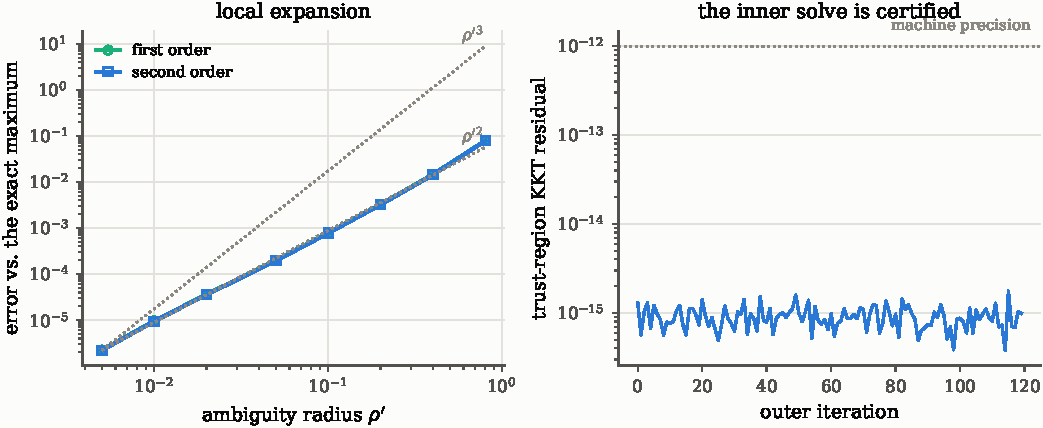
\includegraphics[width=0.9\textwidth]{figs/fig4_theory.pdf}
\caption{Left: error of the local expansion against the exact maximum on the ball, with
the predicted $\rho'^2$ and $\rho'^3$ slopes. Right: the trust-region KKT residual along a
full run of Algorithm~1, flat at machine precision.}
\label{fig:theory}
\end{figure}

\textbf{Latent adversaries dominate data-space adversaries where the loss is nonlinear in
the inputs.} On the short column, worst-case regret is $0.047$ for our method against $0.274$ (PGD,
$5.9\times$) and $0.943$ (WRM, $20\times$) -- the latter more than twice as bad as doing
nothing ($0.389$). On the portfolio there is no such gap: PGD reaches $0.0070$ against our $0.0077$,
and we take that at face value rather than explaining it away. The portfolio's loss depends on $x$
only through the scalar $w^\top x$, so an $L_2$ adversary in data space produces exactly a
mean shift of the return distribution, which is both the dominant held-out shift and a
perturbation with nowhere off-manifold to go. A one-dimensional effective perturbation does
not need a manifold model.

The manifold argument therefore needs stating carefully
(Figure~\ref{fig:manifold}). Pushed to large radii, the data-space adversary on the portfolio reaches
its biggest losses only by driving the mean log-density of its samples $11.9$ nats below
nominal, a likelihood factor of $\sim\!10^5$, certifying against a distribution the true
model effectively rules out. But at the radius where PGD actually performs best
($\epsilon=0.5$) its samples sit $0.00$ nats below nominal, and at comparable damage the
two adversaries pay comparable log-density ($+1.02$ at $1.8$ nats for PGD, $+0.74$ at
$2.0$ nats for ours). The honest claim is not that data-space adversaries are always
off-manifold; it is that they have no mechanism preventing it, so the property has to be
checked per problem, and it fails exactly when the loss depends on the inputs richly enough
for the adversary to have somewhere to go.

\begin{figure}[h]
\centering
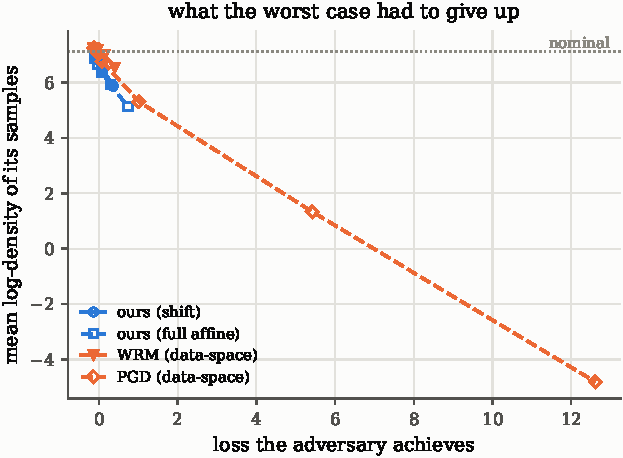
\includegraphics[width=0.9\textwidth]{figs/fig3_manifold.pdf}
\caption{Where each adversary puts its worst case: damage done against how far off the
data manifold it had to go. Read along a curve, not across: at comparable damage the portfolio's
adversaries pay comparable log-density, and the data-space one separates only when pushed
to large radii, where it reaches its biggest losses by driving samples $11.9$ nats below
nominal -- a likelihood factor of $\sim\!10^{5}$ -- certifying against a distribution that
cannot occur. The latent adversary has no setting that leaves the manifold. On the column the data-space adversaries instead
simply stall: the rare-event sigmoid saturates, per-sample gradients vanish, and they
cannot raise the objective past $1.63$ where ours reaches $3.04$.}
\label{fig:manifold}
\end{figure}

\textbf{Simulation cost is modest, and is not the binding constraint.}
Figure~
ef{fig:budget} sweeps the budget, measured in designs actually handed to the true
simulator. The result is that there is nothing to sweep: worst-case regret is flat at
$0.050$--$0.063$ from $M=6$ to $M=128$, with no trend, while over the same range the
surrogate's median relative error on the failure probability falls from $69\%$ to $0.3\%$
-- a factor of $250$. Six simulated designs give a design as good as $128$ do.

The explanation is that the optimizer does not need the surrogate to be accurate, only to
be monotone in the region it searches. A model that misstates $P_f$ by $69\%$ but ranks
nearby designs correctly steers to the same optimum as one that misstates it by $0.3\%$,
because the ranking is what the projected gradient consumes. This is a comfortable property
for the application, where each simulated design is expensive and the surrogate will never
be accurate in absolute terms. It is also a warning: surrogate accuracy is the natural
thing to monitor during fitting and it is nearly uninformative about the quantity we care
about, which is why the validation pass we recommend is against the true loss and not
against held-out surrogate error.

Against a simulator-in-the-loop search charged the same per-design cost we are ahead at
every budget but one, by a median of $1.6\times$ (range $0.9$--$2.0$; the two are level at
$M=16$). The dotted baseline in Figure~\ref{fig:budget} is charged per evaluation instead
and additionally picks its budget split using the held-out metric, so it sits below us at
$0.033$--$0.041$; it is an optimistic bound rather than a method one can run.

\begin{figure}[h]
\centering
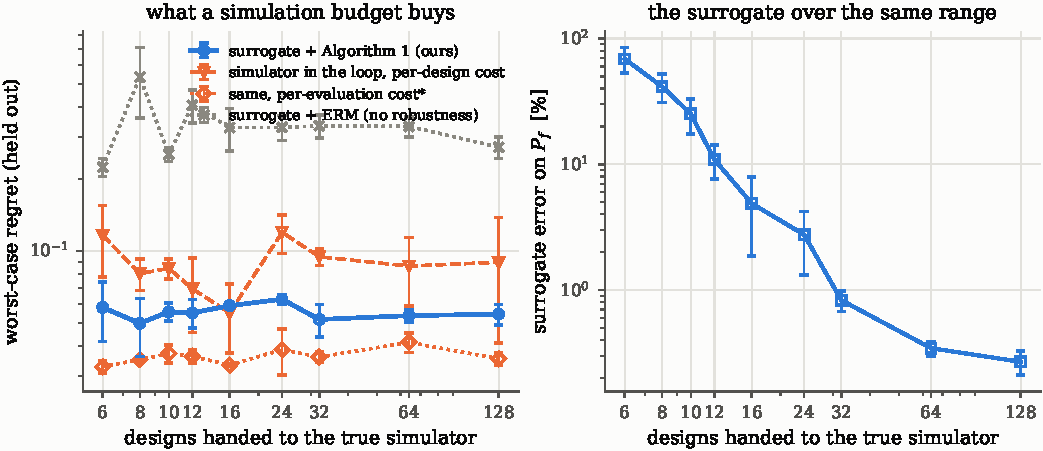
\includegraphics[width=0.9\textwidth]{figs/fig7_budget.pdf}
\caption{Design quality against simulation budget on the short column, against the surrogate's own
accuracy over the same range. Outer iterations of Algorithm~1 are free; only calls to the
true simulator cost anything. Quality is flat while surrogate error falls by a factor of
$250$, so the optimizer is consuming the ranking of designs rather than the predicted
failure probability. The dotted baseline is charged per evaluation rather than per design
and additionally selects its budget split on the held-out metric, so it is an optimistic
bound rather than an achievable method.}
\label{fig:budget}
\end{figure}

\subsection{When the latent set separates, and when it does not}
\label{sec:when}

Table~\ref{tab:results} orders five benchmarks by how much the latent ambiguity set beats
reweighting, and the ordering is not the one we predicted. It is not sorted by how
non-Gaussian the inputs are: the newsvendor has the most non-Gaussian inputs in the suite
and is the only outright loss. It is not sorted by whether the inputs lie on a manifold: the
manifold benchmark gives $1.10\times$, inside one standard error of a tie. The two clear
separations -- the welded beam at $1.47\times$ and DC-OPF at $1.51\times$ -- are the two
problems in which \emph{the adversary has no single direction to push}: four failure modes
that trade off against one another, and a design that must set both a dispatch and who
absorbs the error.

\begin{table}[h]
\centering
\small
\begin{tabular}{llccc}
\toprule
benchmark & the property it isolates & ours & reweighting & ratio \\
\midrule
newsvendor       & non-Gaussian inputs           & $3.873 \pm 0.192$ & $\mathbf{2.909 \pm 0.073}$ & $0.75\times$ \\
short column     & nonlinear loss                & $\mathbf{0.0465 \pm 0.0056}$ & $0.0502 \pm 0.0065$ & $1.08\times$ \\
manifold column  & inputs on a low-dim sheet     & $\mathbf{0.0445 \pm 0.0031}$ & $0.0488 \pm 0.0066$ & $1.10\times$ \\
welded beam      & series system, competing modes & $\mathbf{0.1624 \pm 0.0331}$ & $0.2384 \pm 0.0150$ & $1.47\times$ \\
DC-OPF           & multi-part design             & $\mathbf{0.1178 \pm 0.0124}$ & $0.1777 \pm 0.0115$ & $1.51\times$ \\
\midrule
\emph{portfolio} & \emph{(negative control)}     & $0.0077 \pm 0.0012$ & $0.0074 \pm 0.0005$ & $0.96\times$ \\
\bottomrule
\end{tabular}
\caption{Worst-case regret over held-out shifts at each method's best radius, mean $\pm$
standard error over three seeds; ``reweighting'' is the better of $\chi^2$- and KL-DRO.
Lower is better. The ordering is not by how non-Gaussian the inputs are -- the newsvendor
is the most non-Gaussian benchmark and the worst result -- but by whether the adversary
has a single direction to push. Where the loss has competing failure modes, or the design
trades off several requirements, the latent set separates; where one direction dominates,
it does not.}
\label{tab:results}
\end{table}

\begin{figure}[h]
\centering
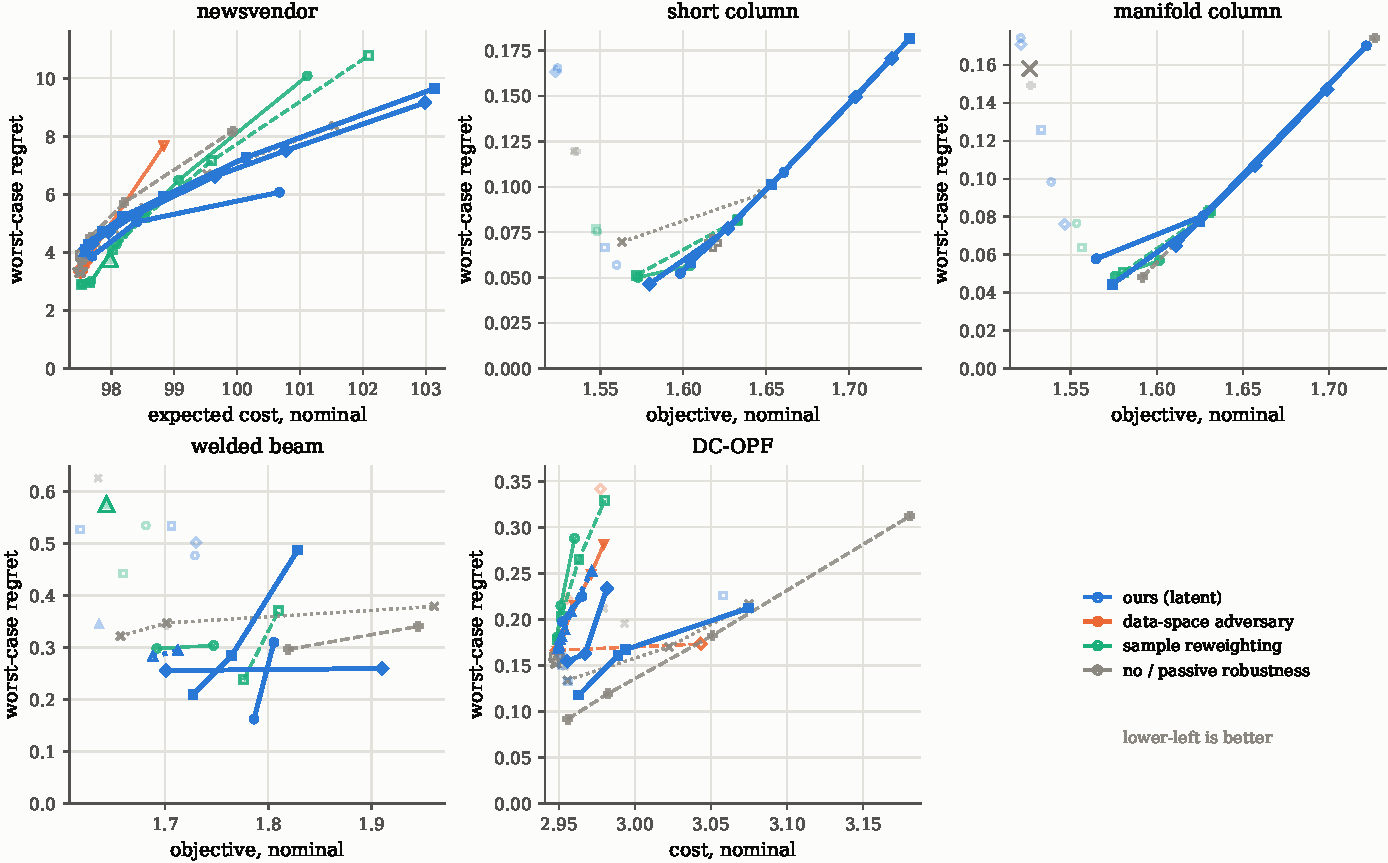
\includegraphics[width=0.9\textwidth]{figs/fig1_frontier.pdf}
\caption{Robustness--performance frontier on each benchmark. Colour encodes the family of
approach; faint markers are every $(\text{nominal}, \text{worst-case})$ pair obtained by
sweeping a method's radius, and the line joins the Pareto-efficient subset. Lower-left is
better. The suite separates into two pictures: where one adversarial direction dominates
(newsvendor, short column, manifold column) the families trace nearly the same frontier;
where several requirements compete (welded beam, DC-OPF) the latent frontier sits below the
others.}
\label{fig:frontier}
\end{figure}

Figure~\ref{fig:frontier} sweeps each method's own radius to trace its whole
robustness--performance frontier rather than the single point of Table~\ref{tab:results}.
On the portfolio every robust method lands between $0.006$ and $0.008$, and the reason is
structural: the portfolio's robust response collapses to a single decision -- how much cash to hold --
so anything inducing the right amount of caution scores the same. Simply raising the
generator's temperature reaches $0.0061$, matching the adversary, and it therefore does
\emph{not} support a claim that the adversary is doing the work. The column does: there the
adversarial version gives $0.047$ against $0.069$ for a random latent perturbation of the
same divergence and $0.069$ for a broadened generator, a $1.5\times$ separation that holds
across seeds. What it still separates cleanly is robustness of any kind from none, since
ERM gives $0.046$ and a random latent shift gives $0.040$ -- that is, passive perturbation
of a \emph{correctly fitted} generator buys essentially nothing.

We think the mechanism is this. A reweighting set and a latent set both have a most
efficient attack, and when one direction dominates the objective they find the same one --
which is why the portfolio, whose loss is a single linear functional of the inputs, is a
tie at $0.96\times$, and why a data-space $L_2$ adversary is competitive there too. When
several requirements compete, the worst case is a \emph{joint} configuration rather than a
direction: enough load to stress the weld without relieving the deflection mode, correlated
across inputs. A latent transformation expresses that as one affine map; reweighting must
find sample points that already happen to realise it. That is a statement about the loss
and the design, not about the input distribution, which is why non-Gaussianity alone buys
nothing.

The newsvendor deserves its own sentence, since it is the one outright loss and the
obvious suspect is the generator. That suspect is half right. Plain ERM on flow samples
scores $3.89$ there against $3.36$ on the real sample, so merely \emph{sampling} from the
generator costs $0.53$ before any adversary acts. But replacing it with an oracle -- a flow
fitted to $200{,}000$ true samples, $\mathrm{KL}(P\|p_\theta)=0.036$ -- improves our
worst-case regret only from $4.12$ to $3.62$, still well behind KL-DRO's $2.86$. Half the
deficit is generator quality and half is the ambiguity set: a worst case that moves mass
between two well-separated modes is what reweighting does trivially and a smooth latent map
does badly.

The practical reading for the muon shield is favourable and specific: $43$ design
parameters and many independent leakage routes is the multi-mode, multi-part regime, not
the single-direction one.

\begin{remark}[The manifold argument is about the certificate, not the ranking]
\label{rem:manifold}
We built the manifold benchmark expecting data-space adversaries to collapse on it, and
they do not collapse any harder than on the ordinary column: PGD is $4.3\times$ worse than
us with the inputs on a sheet and $5.9\times$ worse without. The reason is worth recording,
because it corrects the natural reading of Figure~\ref{fig:manifold}. Held-out regret is
computed under real shifts, and real shifts move only the physical coordinates. An
adversary that wanders off the sheet is describing inputs that cannot occur -- its
\emph{certificate} is void -- but nothing forces the design it returns to be bad. Leaving
the manifold invalidates the guarantee; it does not automatically cost design quality. The
log-density measurements are the evidence for the manifold claim, and a regret table is not.
\end{remark}

\subsection{Where it separates: small samples}
\label{sec:smallsample}

Table~\ref{tab:results} is measured with a comfortable training sample. The gap that opens
when data is scarce is larger than any of those ratios and in the same direction on every
benchmark, which is the regime the construction was built for: reweighting can only move
mass between points it has already seen, while a fitted generator puts mass between them.
Sweeping the sample every method is given, on the short column, with three seeds
(Figure~\ref{fig:smallsample}):

\begin{center}\small
\begin{tabular}{lcccccc}
\toprule
$n$ & 50 & 100 & 200 & 500 & 2000 & 8000 \\
\midrule
ERM               & 1.092 & 1.125 & 0.714 & 0.403 & 0.382 & 0.351 \\
$\chi^2$-DRO      & 0.607 & 0.986 & 0.533 & 0.125 & 0.085 & \textbf{0.043} \\
KL-DRO            & 0.578 & 0.966 & 0.535 & 0.127 & 0.085 & \textbf{0.042} \\
latent-DRO (ours) & \textbf{0.037} & \textbf{0.134} & \textbf{0.051} & \textbf{0.047} & \textbf{0.053} & 0.054 \\
\bottomrule
\end{tabular}
\end{center}

Our worst-case regret is flat in $n$ -- $0.037$ to $0.134$ over a $160\times$ range -- while
reweighting degrades by a factor of $14$ from $n=8000$ down to $n=50$. At $n=50$ the gap is
$16\times$; the curves cross near $n\approx2000$, past which reweighting is slightly
better. The portfolio shows the same shape less sharply ($0.016$ against $0.120$ for
$\chi^2$-DRO at $n=50$).

The newsvendor is the exception, and it is an exception at every sample size rather than a
crossover: $4.94$ against $3.30$ for KL-DRO at $n=50$, $3.76$ against $3.49$ at $n=8000$.
Its generator is the worst in the suite at small $n$ -- $\mathrm{KL}(P\|p_\theta) = 6.1$ at
$n=50$, against radii of $0.05$--$0.3$ -- so the ambiguity set is centred somewhere the
data is not, and no radius repairs that. The claim this section supports is therefore
conditional, and the condition is the one Remark~\ref{rem:prior} already names: the
generator has to be good enough that its own divergence from the truth is small next to the
radius being swept. Where that holds the small-sample advantage is large; where it does not,
there is no advantage to have. This is the property that matters for the shield, where operating
conditions come from an expensive simulator rather than being collected cheaply.

\begin{figure}[h]
\centering
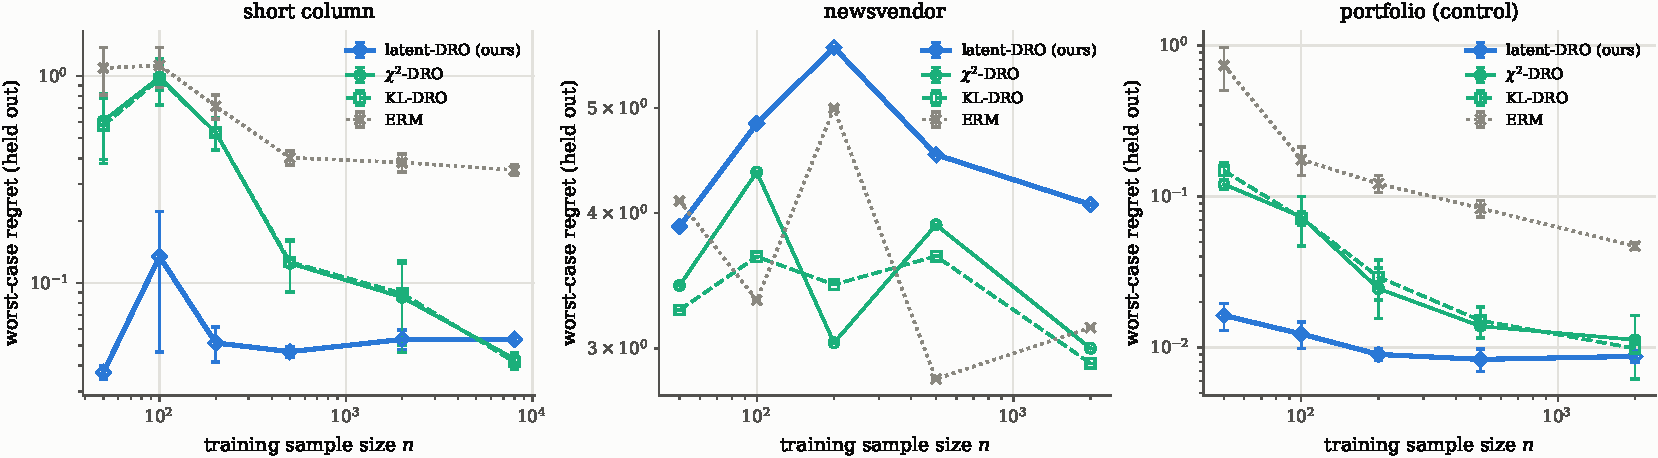
\includegraphics[width=0.92\textwidth]{figs/fig9_smallsample.pdf}
\caption{Worst-case regret against the size of the training sample every method is given.
On the short column our curve is nearly flat while reweighting and ERM climb steeply as
data becomes scarce -- reweighting can only redistribute mass among points it has seen. The
newsvendor is the exception and stays an exception at every sample size, for the reasons in
Section~\ref{sec:when}. The spike at $n=100$ on the column is one seed of three.}
\label{fig:smallsample}
\end{figure}

\begin{remark}[What is doing the work is smoothness, not flow expressiveness]
\label{rem:prior}
It is tempting to read the above as evidence that flows learn efficiently from little
data. They do not. Measuring $\mathrm{KL}(P \,\|\, p_\theta)$ against the analytic density,
a flow fitted to $50$ samples scores $0.33$ on the column while a flow given \emph{no gradient
steps at all} -- only the ActNorm data initialisation, which is a diagonal Gaussian matched
to the sample's marginals -- scores $0.24$. At $n \le 200$, on both benchmarks, fitting the
flow is worse than not fitting it. Our method wins at $n=50$ while anchored to a generator
that is worse than its own initialisation, so what it is exploiting is the smoothness of
\emph{any} parametric density model, not the expressiveness of this one. Two consequences:
a simpler generator would serve at small $n$, and the benchmark on which the flow earns its
keep is one where the Gaussian prior is wrong -- the column, where fitting improves
$\mathrm{KL}$ from $0.156$ to $0.024$ at $n=2000$, and not the portfolio, where it changes
nothing ($0.079$ against $0.081$) -- which is why the portfolio is reported here only as a
control.
\end{remark}

\subsection{The radius is interpretable, and unbounded}
\label{sec:radius}

Two properties are specific to this construction. First, by
Proposition~\ref{prop:invariance} the radius $\rho$ is a divergence in data space, so it can
be compared against the divergence of a real shift. On the portfolio the best radius is
$\rho\approx0.05$--$0.15$ against held-out shifts at true KL divergences of $0.18$--$0.67$;
on the column, $\rho\approx0.15$--$0.3$ against $0.22$--$2.38$. The useful radius is a
factor of two to four \emph{below} the shifts it defends against, which is the expected
direction -- the worst distribution at radius $\rho$ is more damaging than any particular
real shift of the same divergence -- and the point is that the two are on the same scale and
can be calibrated against each other. A reweighting radius admits no such comparison, since
it measures a divergence between weightings of one sample rather than between
distributions.

\begin{remark}[Reweighting radii have a ceiling; latent radii do not]
\label{rem:ceiling}
The second property is a limit that applies to the reweighting baselines and not to us. On
a fixed sample of size $n$, the most divergent admissible reweighting is the one supported
on whichever points attain the maximum loss. For a $0/1$ loss with a failing fraction $q$
this caps the achievable divergence at $\mathrm{KL}=\log(1/q)$, or
$\chi^2=(1/q-1)/2$; CVaR at level $\alpha$ degenerates once $\alpha\le q$, its tail average
being taken entirely inside the failure set. On the column at the shared starting design
$q=0.375$, giving caps of $0.98$, $0.83$ and $0.38$ respectively. Beyond the cap the constraint stops binding, the reweighted risk saturates
at $\max_i \ell_i$, and its gradient in $\design$ collapses to whatever part of the
objective does not depend on the sample -- on the column the cross-sectional area, so the optimizer
shrinks the column until it fails with probability one. We observe exactly this: every
radius past the cap returns the same degenerate design, and the transition is bracketed
exactly where the cap predicts for all three tail-based baselines:

\begin{center}\small
\begin{tabular}{lccc}
\toprule
 & predicted cap & last good setting & first degenerate setting \\
\midrule
KL-DRO       & $\log(1/q)=0.98$   & $\rho=0.6$: $0.082$ & $\rho=1.2$: $8.80$ \\
$\chi^2$-DRO & $(1/q-1)/2=0.83$   & $\rho=0.4$: $0.056$ & $\rho=1.0$: $8.80$ \\
CVaR         & $\alpha\le q=0.38$ & $\alpha=0.5$: $0.203$ & $\alpha=0.3$: $8.80$ \\
\bottomrule
\end{tabular}
\end{center}

\noindent The latent set has no analogous ceiling: every $\eta$ in the ball yields a proper
distribution over inputs however large $\rho$ grows. This does not affect
Table~\ref{tab:results}, where each method gets its best radius, but the reweighting
baselines are only defined over part of the range the sweep covers.
\end{remark}

\subsection{Every method, iteration by iteration}

Table~\ref{tab:results} reports where each method ends up. Figure~\ref{fig:trajectory}
reports how it gets there, on equal terms: every method starts from the same design, and at
each iteration recomputes whatever its own ambiguity set says the worst case is -- the
generator is fixed throughout -- and takes one projected step. Solid curves are the nominal
loss, dashed the worst case over held-out shifts.

Three things are visible that a table cannot show. All methods converge within about $25$
iterations, so no comparison is confounded by one being stopped early. The ordering of the
solid curves is the reverse of the dashed ones -- every robust method buys its worst case
with nominal loss, and ours pays the most. And our nominal curve oscillates where the
others are smooth, because the adversary is re-solved each step and the design chases a
moving target; the oscillation is confined to the nominal loss, while the worst case being
optimized is stable.

The figure is drawn on the portfolio control, where PGD wins at $-0.116$ against our
$-0.113$ -- an instructive case rather than an anomaly. That loss depends on $x$ only
through $R=w^\top x$, so an $L_2$ ball in data space produces exactly a downward mean shift,
which is the form the dominant held-out shifts take: the data-space adversary is close to
well specified, and its one-dimensional effective perturbation has nowhere off-manifold to
go. It is the clearest illustration of Section~\ref{sec:when}: where a single direction
dominates, every ambiguity set finds it and none can separate.

\begin{figure}[h]
\centering
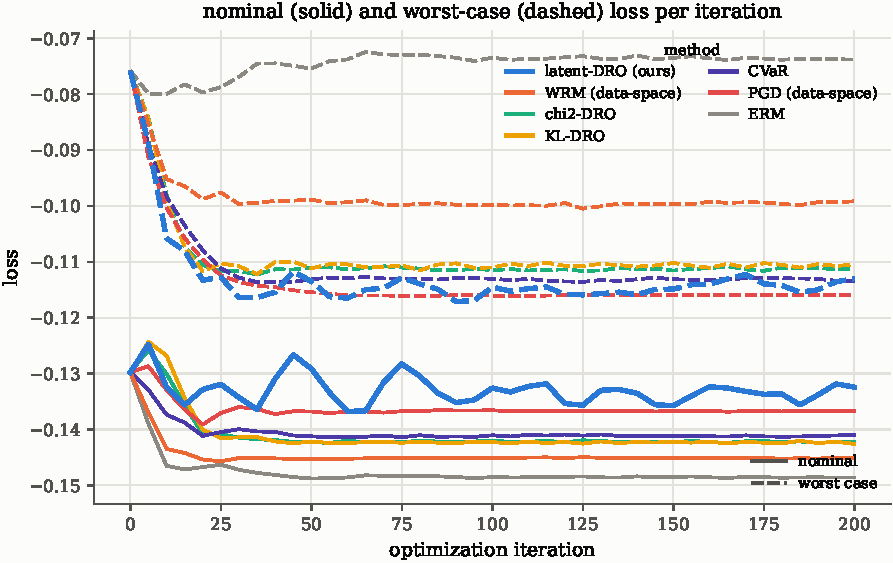
\includegraphics[width=0.85\textwidth]{figs/fig10_trajectory.pdf}
\caption{Nominal (solid) and worst-case (dashed) loss at each outer iteration on the portfolio control, every
method from the same starting design and at its own best radius. Lower is better. All
methods converge within $\sim25$ iterations. PGD attains the lowest worst-case loss on this
problem and ours the third lowest; see the text for why it favours a data-space adversary.
Our nominal curve is the highest of the robust methods, which is the price being paid.}
\label{fig:trajectory}
\end{figure}

\begin{figure}[h]
\centering
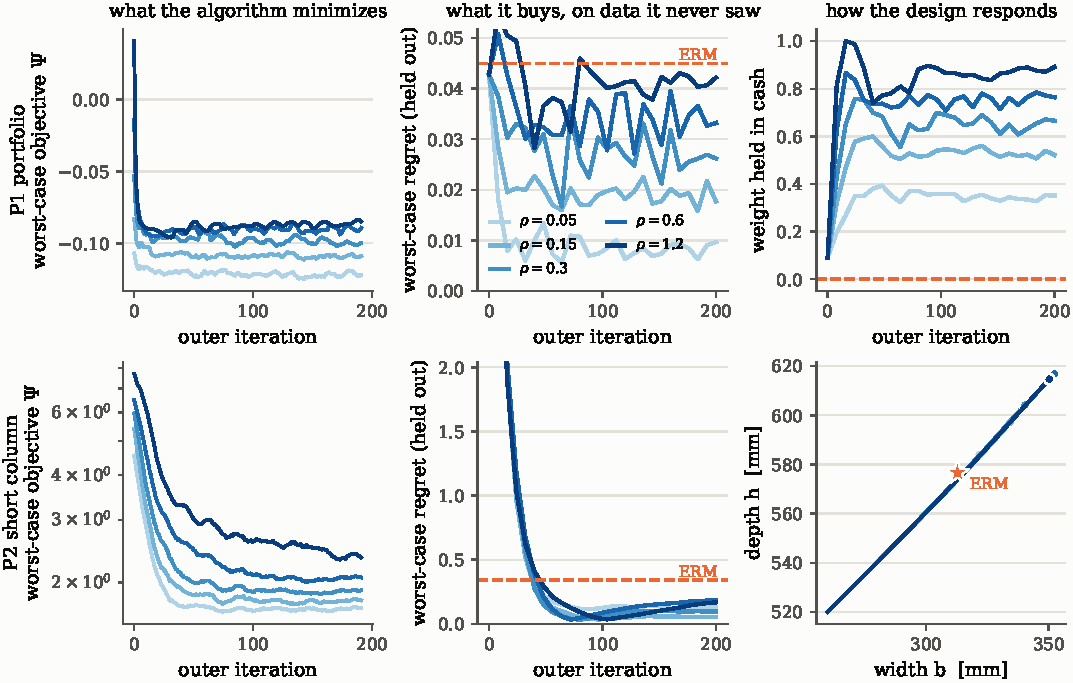
\includegraphics[width=0.95\textwidth]{figs/fig6_progress.pdf}
\caption{Progress of Algorithm~1 at five radii (light to dark). Left: the minimax
objective, the only signal the algorithm sees. Middle: worst-case regret on held-out
shifts, which it never observes -- note that on the column it bottoms out near iteration 60--80 and
then degrades. Right: the design response, cash weight on the portfolio and the path through $(b,h)$
on the column.}
\label{fig:progress}
\end{figure}

Held-out regret does not decrease monotonically with optimization, and this is the one
place where running Algorithm~1 to convergence is actively harmful. On the short column it reaches its
minimum around outer iteration $70$--$100$ and then \emph{rises} while the training
objective keeps improving: at $\rho=0.6$ from $0.032$ to $0.183$, a factor of $5.8$, and at
$\rho=0.3$ from $0.033$ to $0.095$. The same happens more mildly on the portfolio. The algorithm is
converging on the surrogate's minimax problem and drifting away from what generalizes --
the surrogate-error term of Section~\ref{sec:theory} again, accumulating with iteration
count rather than with dimension.

This is worth being concrete about, because it means our own headline numbers are
conservative and honestly so. Table~\ref{tab:results} reports the design after a fixed
$200$ iterations for every method; stopping the column at its best iterate instead would give
$0.033$ rather than $0.047$. We do not report that number as the result, because choosing
the stopping point requires the held-out shifts the metric is computed on, and no user has
them. What a user does have is the option to hold out a shift they can afford to simulate,
which on this evidence is worth more than any other tuning decision in the pipeline.

% ============================================================================
\section{Conclusion}
% ============================================================================
By intersecting normalizing flows with branch--trunk surrogates, we make DRO tractable for
expensive simulators: mapping the ambiguity set to a latent Euclidean ball bypasses optimal
transport, the inner problem becomes an exactly solvable trust-region subproblem, and the
whole optimization runs without touching the simulator. The machinery works -- it recovers
brute-force ground truth to $0.35\%$, its inner certificate holds to $10^{-15}$, and it
needs remarkably little simulation.

Whether it is \emph{worth} the machinery is a separate question, and most of this paper is
about answering it honestly. Against sample reweighting the verdict depends on the problem
in a way we can now state: the latent set separates when several requirements compete, so
that the worst case is a joint configuration rather than a direction ($1.47\times$ on a
series system, $1.51\times$ on a two-part power-flow design), and ties or loses when one
direction dominates the loss. Non-Gaussian inputs, which we expected to be the deciding
property, decide nothing: the most non-Gaussian benchmark in the suite is the one we lose,
and an oracle generator recovers only half of that deficit. The remaining half is the
ambiguity set being the wrong shape for a worst case that moves mass between two separated
modes -- easy to reweight, hard to reach by a smooth latent map.

Two advantages are independent of that question. Reweighting degrades by a factor of $14$ as
the sample shrinks from $8000$ points to $50$ while our worst-case regret stays flat, because
it can only move mass between points it has already seen. And a reweighting radius has a hard
ceiling on a bounded loss, beyond which the baseline degenerates entirely, which a latent
radius does not. Both matter for the muon shield, where operating conditions are known
through an expensive model rather than a cheap covering sample.

We are explicit about what we could not establish. The second-order expansion does not attain
its predicted cubic order on either benchmark where we can measure it
(Section~\ref{sec:theory-emp}); the manifold benchmark we built to test the
method's central premise supports it only through the log-density diagnostic and not through
design quality (Remark~\ref{rem:manifold}); and two benchmarks turn out not to test the
generative model at all. The shield is $43$-dimensional with many independent leakage routes,
which is the regime our results favour -- but settling that requires the application rather
than another proxy.

\bibliographystyle{plainnat}
\bibliography{references} 

% Note: Replace with actual bib items as in your original draft if not using a separate .bib file.
\begin{thebibliography}{9}

\bibitem{ben-tal2009} A. Ben-Tal, L. El Ghaoui, A. Nemirovski. \emph{Robust Optimization.} Princeton University Press, 2009.
\bibitem{esfahani2018} P. Mohajerin Esfahani, D. Kuhn. \emph{Data-driven distributionally robust optimization using the Wasserstein metric...} Mathematical Programming, 2018.
\bibitem{sinha2018} A. Sinha, H. Namkoong, J. Duchi. \emph{Certifying some distributional robustness with principled adversarial training.} ICLR, 2018.
\bibitem{lu2021} L. Lu, P. Jin, G. Pang, Z. Zhang, G. E. Karniadakis. \emph{Learning nonlinear operators via DeepONet...} Nature Machine Intelligence, 2021.
\bibitem{scarf1958} H. Scarf. \emph{A min-max solution of an inventory problem.} In Studies in the Mathematical Theory of Inventory and Production, Stanford University Press, 1958.
\bibitem{kuschel1997} N. Kuschel, R. Rackwitz. \emph{Two basic problems in reliability-based structural optimization.} Mathematical Methods of Operations Research, 1997.
\bibitem{ragsdell1976} K. M. Ragsdell, D. T. Phillips. \emph{Optimal design of a class of welded structures using geometric programming.} Journal of Engineering for Industry, 1976.
\bibitem{youn2004} B. D. Youn, K. K. Choi. \emph{An investigation of nonlinearity of reliability-based design optimization approaches.} Journal of Mechanical Design, 2004.
\bibitem{bienstock2014} D. Bienstock, M. Chertkov, S. Harnett. \emph{Chance-constrained optimal power flow: risk-aware network control under uncertainty.} SIAM Review, 2014.
\bibitem{roald2015} L. Roald, G. Andersson. \emph{Chance-constrained AC optimal power flow: reformulations and efficient algorithms.} IEEE Transactions on Power Systems, 2018.
\bibitem{delage2010} E. Delage, Y. Ye. \emph{Distributionally robust optimization under moment uncertainty with application to data-driven problems.} Operations Research, 2010.
\bibitem{shirobokov2020} S. Shirobokov, V. Belavin, M. Kagan, A. Ustyuzhanin, A. G. Baydin. \emph{Black-box optimization with local generative surrogates.} Advances in Neural Information Processing Systems (NeurIPS), 2020.
\bibitem{dinh2017} L. Dinh, J. Sohl-Dickstein, S. Bengio. \emph{Density estimation using Real NVP.} International Conference on Learning Representations (ICLR), 2017.
\bibitem{kingma2018} D. P. Kingma, P. Dhariwal. \emph{Glow: generative flow with invertible $1\times1$ convolutions.} Advances in Neural Information Processing Systems (NeurIPS), 2018.
\bibitem{rezende2015} D. J. Rezende, S. Mohamed. \emph{Variational inference with normalizing flows.} International Conference on Machine Learning (ICML), 2015.
\bibitem{durkan2019} C. Durkan, A. Bekasov, I. Murray, G. Papamakarios. \emph{Neural spline flows.} Advances in Neural Information Processing Systems (NeurIPS), 2019.
\bibitem{papamakarios2021} G. Papamakarios, E. Nalisnick, D. J. Rezende, S. Mohamed, B. Lakshminarayanan. \emph{Normalizing flows for probabilistic modeling and inference.} Journal of Machine Learning Research, 2021.
\bibitem{namkoong2016} H. Namkoong, J. C. Duchi. \emph{Stochastic gradient methods for distributionally robust optimization with $f$-divergences.} Advances in Neural Information Processing Systems (NeurIPS), 2016.
\bibitem{duchi2021} J. C. Duchi, H. Namkoong. \emph{Learning models with uniform performance via distributionally robust optimization.} The Annals of Statistics, 2021.
\bibitem{kuhn2019} D. Kuhn, P. Mohajerin Esfahani, V. A. Nguyen, S. Shafieezadeh-Abadeh. \emph{Wasserstein distributionally robust optimization: theory and applications in machine learning.} INFORMS TutORials in Operations Research, 2019.
\bibitem{more1983} J. J. Mor\'e, D. C. Sorensen. \emph{Computing a trust region step.} SIAM Journal on Scientific and Statistical Computing, 1983.
\bibitem{danskin1967} J. M. Danskin. \emph{The Theory of Max-Min and its Application to Weapons Allocation Problems.} Springer, 1967.

\end{thebibliography}

\end{document}